\documentclass[document.tex]{subfiles}
\begin{document}
	
\chapter{Introduction}

\section{Overview}
\noindent Hyperspectral sensors simultaneously measure hundreds of continuous spectral bands with a fine resolution to form a three dimensional hyperspectral image data cube. For instance, the AVIRIS sensor simultaneously measures 224 bands with a fine resolution of 0.01$\mu$m. This high data volume presents many challenges which creates opportunity for research. The data captured are highly correlated and contains a significant amount of redundant data. All the image bands are not equally important for specific application.  Also, as the feature space dimension increases, if the size of the training data does not grow correspondingly, a reduction in the classification accuracy of the testing data is observed due to poor parameter estimation of the supervised classifier. This effect is known as the Hughes phenomenon\cite{1}. So it is required to extract only relevant features from the input dataset. Therefore an effective and efficient technique to find this relevant features is a major interest in current literature. Principal component analysis (PCA)\cite{7} is one of the most popular feature extraction technique, though its components is not always suitable for better classification accuracy\cite{8}. It is also not sensitive to input classes and consider only the global variance of the dataset. There are few techniques for finding relevant features in current literature. For example, mutual information based feature selection in combination of principal component analysis\cite{10} and normalized mutual information based feature selection\cite{9}. A target class oriented subspace detection technique (TCOSD) is proposed as an alternative for the effective subspace detection in collaboration with kernel support vector machine (SVM)\cite{11} to achieve better classification accuracy.

\clearpage  

\section{Remote Sensing}
\noindent Remote sensing is the acquisition of information about an object or phenomenon without making physical contact with the object. Remote sensing is used in numerous fields, including geography, land surveying and most Earth Science disciplines (for example, hydrology, ecology, oceanography, glaciology, geology); it also has military, intelligence, commercial, economic, planning, and humanitarian applications.

\begin{figure}[H]
	\begin{center}
		\includegraphics[height=7.0cm]{imgs/Active.png}
	\end{center}
	\caption{Active remote sensing\cite{32}}
	\label{fig: Active remote sensing}
\end{figure}
\vline
\begin{figure}[H]
	\begin{center}
		\includegraphics[height=7.0cm]{imgs/Passive.png}
	\end{center}
	\caption{Passive remote sensing\cite{32}}
	\label{fig: Passive remote sensing}
\end{figure}

\noindent In current usage, the term "remote sensing" generally refers to the use of satellite- or aircraft-based sensor technologies to detect and classify objects on Earth, including on the surface and in the atmosphere and oceans, based on propagated signals (e.g. electromagnetic radiation). It may be split into "active" remote sensing (i.e., when a signal is emitted by a satellite or aircraft and its reflection by the object is detected by the sensor) and "passive" remote sensing (i.e., when the reflection of sunlight is detected by the sensor). Fig. \ref{fig: Active remote sensing} and Fig. \ref{fig: Passive remote sensing} shows a scenario with active and passive remote sensing platform. Fig. \ref{fig: Hyperspectral cube} presents a 3D view of data obtained by these sensors.
\begin{figure}[H]
	\begin{center}
		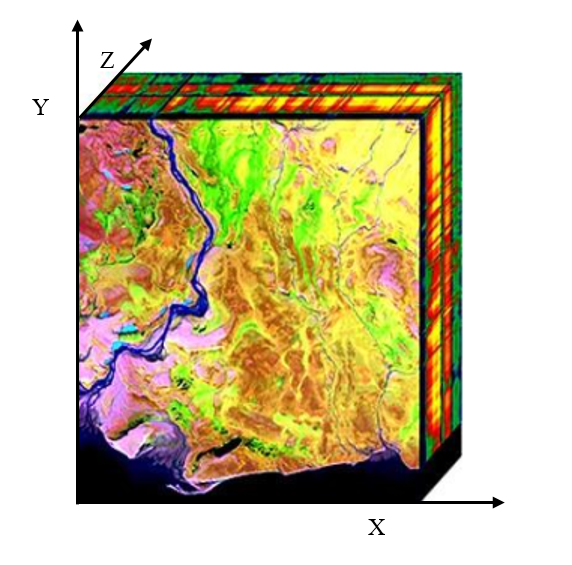
\includegraphics[height=10.0cm]{imgs/cube.png}
	\end{center}
	\caption{Hyperspectral data cube (3D view)\cite{31}}
	\label{fig: Hyperspectral cube}
\end{figure}

%\section{Challenges of Remote Sensing}
%%\noindent Hyperspectral imaging is a popular field of remote sensing. The main challenge of hyperspectral image is its highly correlated huge data set. On the other hand, this large number of spectral bands has a direct impact on the required computational cost for classification. Also, as the feature space dimension increases, if the size of the training 
%\noindent As we have entered an era of high resolution earth observation, the RS data are undergoing an explosive growth. The proliferation of data also give rise to the increasing complexity of RS data, like the diversity and higher dimensionality characteristic of the data. RS data are regarded as RS “Big Data”. In ground object detection, remote sensing faces several challenges. A few challenges of remote sensing in ground object detection is given below:
%\begin{itemize}
%	\item Field sampling is difficult and expensive
%	\item The geographical orientation is difficult in the images
%	\item The upwelling signal to the sensor is low and disturbed
%	\item The water and its constituents limits the usable spectral region
%\end{itemize}
%
%\begin{figure}[H]
%	\begin{center}
%		\includegraphics[height=8.0cm]{imgs/capture.png}
%	\end{center}
%	\caption{Technical characteristics of
%		digital image data\cite{3}}
%	\label{fig: Technical characteristics of
%		digital image data}
%\end{figure}
%
%% \noindent data does not grow correspondingly, a reduction in the classification accuracy of the testing data is observed due to poor parameter estimation of the supervised classifier. This effect is known as the Hughes phenomenon\cite{1}.
%\noindent Fig. 1.4 represents the technical characteristics of the digital data form of reflections received by the remote sensing sensors.

\section{Challenges of Hyperspectral Data Processing}
Optical sensing has come a long way from grayscale to multispectral and now to hyperspectral images. The advances in imaging hardware over recent decades have enabled availability of high spatial, spectral, and temporal resolution imagery for a variety of applications. Hyperspectral imagery, also
called imaging spectroscopy, entails acquiring images using a
large number (typically a few hundreds) of narrow and often
contiguous spectral bands, covering a wide range of the electromagnetic spectrum from the visible to the infrared regions.
Compared to conventional color imagery (with 3 spectral bands
covering the red, green and blue wavelengths, respectively),
or compared to conventional multispectral imagery (typically
a few spectral bands), hyperspectral data provide a very fine
spectral characterization of the sensed materials, which facilitates their detection and characterization. Advances in hardware to acquire hyperspectral imagery have
made such data easily accessible to a wide variety of application domains, but have also created unique challenges for
researchers working on algorithms for the representation, exploitation, and analysis of such data. Unfortunately, this is often
a double-edged sword. A direct consequence of the dense spectral sampling implies that each measurement corresponds to a
vector with several hundreds of values. Consequently, the data
are evolving in a vector space with several hundreds of dimensions. Traditional information-processing techniques cannot be
used to process such data effectively. While it is a curse from an
analytical, theoretical, and statistical point of view, the very high
dimensionality of the data is also a blessing. But the main challenge of hyperspectral image is its highly correlated huge data set. On the other hand, this large number of spectral bands has a direct impact on the required computational cost for classification. Also, as the feature space dimension increases, if the size of the training data does not grow correspondingly, a reduction in the classification accuracy of the testing data is observed due to poor parameter estimation of the supervised classifier. This effect is known as the Hughes phenomenon\cite{1}. Challenges of hyperspectral images are given below:
\begin{itemize}
	\item Curse of dimensionality.
	\item High correlation.
	\item Irrelevant information for classification.
\end{itemize}


\begin{figure}[H]
\begin{center}
	\includegraphics[height=8.0cm]{imgs/curse.png}
\end{center}
\caption{Curse of dimensionality\cite{9}}
\label{fig:Curse of dimensionality}
\end{figure}
\noindent In Fig. \ref{fig:Curse of dimensionality} the problem of hyperspectral data, curse of dimensionality is present in image band number 35. From image band 35, the accuracy of the classification task is gradually decreasing as the train sample of the experiment remains constant. Fig. \ref{fig:Correlation among bands of AVIRIS data set} shows correlations among bands of AVIRIS 92AV3C data set. Here white color means 100\% correlated and Black means 0\% correlation.
\begin{figure}[H]
	\begin{center}
		\includegraphics[height=8.0cm]{imgs/corr.png}
	\end{center}
	\caption{Correlation among bands of AVIRIS data set}
	\label{fig:Correlation among bands of AVIRIS data set}
\end{figure}
\section{Motivation}
\noindent Hyperspectral image processing is  one of the fast growing research field because of its various applications. Remotely sensed ground areas are classified into different groups of object by classification of the hyperspectral image. For this purpose, feature extraction and selecting only relevant features before classification is an important task to achieve high classification accuracy. So effective subspace detection is very important for classification of hyperspectral images. Few motivation for this research is given below:
\begin{itemize}
	\item Extract only relevant features and find an effective subspace
	\item Address curse of dimensionality\cite{1}
	\item Improve classification accuracy
\end{itemize}

\section{Objectives}
\noindent The main objective of this research work is to illustrate a target class oriented subspace detection method (TCOSD) which is a combination of feature extraction using principal component analysis (PCA) and relevant feature selection by normalized mutual information (NMI) to achieve a better classification accuracy. Objectives of this research will be:
\begin{itemize}
	\item Create a method of feature extraction by removing correlation among bands.
	\item Create an approach to select relevant features after feature extraction.
	\item Create a method with collaboration of feature mining and classification.
	\item Improving classification accuracy.
\end{itemize}

\section{Outline}
\noindent This report is organized in 5 chapters discussing all related topics that may be helpful in reproducing a subspace method for effective ground object detection and identification.
\begin{itemize}	
\item \textbf{Chapter 1:} A short overview of the whole research work and topics related to this research is discussed in this chapters.
\item \textbf{Chapter 2:} Basics of hyperspectral remote sensing, sensors, applications and problems of hyperspectral images are discussed in this chapter. 
\item \textbf{Chapter 3:} This chapter is focused on the current literature of this research field. Recent and relevant feature mining techniques are discussed in this chapter.
\item \textbf{Chapter 4:} Features extraction based on PCA and relevant features selection using NMI, their implementation with experimental results on real hyperspectral image is discussed in this chapter. Details explanations, algorithm, flow chart and experimental results of our proposed target class oriented subspace detection method (TCOSD) is also discussed in this chapter. Chapter 4 is the main part of this thesis report book.
\item \textbf{Chapter 5:} Conclusion of this research is noted in this chapter. Drawbacks of the proposed TCOSD method and possible ways of improvement is also discussed here.
\end{itemize}
\end{document}
